\documentclass[oneside,12pt]{Classes/aesm_edspia}


\usepackage[utf8x]{inputenc}
\usepackage{minitoc}
\usepackage[latin1]{inputenc}
\usepackage[french]{babel}
\usepackage[T1]{fontenc}
\usepackage{amsmath}
\usepackage{lmodern}%font modern
\rmfamily
\DeclareFontShape{T1}{lmr}{bx}{sc}{<->ssub * cmr/bx/sc}{} 
\usepackage{lettrine}
\usepackage{tabularx}
\usepackage[utf8x]{inputenc}
\usepackage{epsfig, floatflt, amssymb} 
\usepackage{moreverb} %% pour le verbatim en boite
\usepackage{cases}%equations en systemes numérotés - soluce possible package : CASES
\usepackage{multirow} %% pour regrouper un texte sur plusieurs lignes dans une table
\usepackage{url} %% pour citer les url par \url
\usepackage[all]{xy} %% pour la barre au dessus des symboles
\usepackage{textcomp} %% pour le symbol pour mille par \textperthousand et degrés par \degres
\usepackage[right]{eurosym}
\usepackage{setspace} %interligne simple, double etc...
\usepackage{Classes/eurosans} %%pour le symbole \euro
\usepackage{epic,eepic}
\usepackage{soul}
\usepackage[nottoc]{tocbibind} % tables des figures, des matieres et autres dans la TOC
\usepackage{fancybox}
\usepackage[leftcaption]{sidecap}
\usepackage[labelsep=endash, textfont={footnotesize, singlespacing}, margin=10pt, format=plain, labelfont=bf]{caption}
\usepackage[Conny]{Classes/fncychap} %en tete chapitrage
\newcommand{\ie}{c.-\`a-d.~}
\hbadness=10000% pb d'overfull box réglé
\hfuzz=50pt
\pdfcompresslevel9 % pour compresser le pdf final au maximum
\pdfoptionpdfminorversion=5 % pour accepté les images PDF version 1.5 (ex: celles produites par Office 2007)
\def\underscore{\char`\_}
\makeatletter
\renewcommand{\thesection}{\arabic {section}}
\renewcommand{\SC@figure@vpos}{c}% centrer verticalement le caption avec le package sidecap...
\renewcommand{\fnum@figure}{\small\textbf{Figure~\thefigure}}
\renewcommand{\fnum@table}{\small\textbf{Tableau~\thetable}}

\makeatother
\usepackage{subfig}
\def\thechapter{\Roman{chapter}}

\usepackage[framed,numbered,autolinebreaks,useliterate]{Classes/mcode}


%%% Listings

\usepackage{listings}
\lstloadlanguages{xml, java}
	
	 \usepackage{listings}
  \usepackage{courier}
 \lstset{
         basicstyle=\footnotesize\ttfamily, 
         %numbers=left,               
         numberstyle=\tiny,          
         %stepnumber=2,               
         numbersep=5pt,              
         tabsize=2,                  
         extendedchars=true,         
         breaklines=true,            
         keywordstyle=\color[rgb]{0.43,0,0}\textbf,
    		frame=b,
         commentstyle=\color[rgb]{0.51,0.51,0.51} \textit ,
         stringstyle=\ttfamily  \color[rgb]{0,0.44,0} ,
         showspaces=false,           
         showtabs=false,             
         xleftmargin=17pt,
         framexleftmargin=17pt,
         framexrightmargin=5pt,
         framexbottommargin=4pt,
         %backgroundcolor=\color{lightgray},
         showstringspaces=false            
 }
 
 \usepackage{caption}
\DeclareCaptionFont{white}{\color{white}}
\DeclareCaptionFont{red}{\color{red}}
\DeclareCaptionFont{black}{\color{black}}
\DeclareCaptionFormat{listing}{\colorbox[cmyk]{0.43, 0.35, 0.35,0.01}{\parbox{\textwidth}{\hspace{15pt}#1#2#3}}}
\captionsetup[lstlisting]{format=listing,labelfont=black,textfont=white, singlelinecheck=false, margin=0pt, font={bf,footnotesize}}


%%%%%%%%%%%%%%%%%%%%%%%%%%%%%%%%%%%%%%%%%%%
\begin{document}
%%%%%%%%%%%%%%%%%%%%%%%%%%%%%%%%%%%%%%%%%%%
\renewcommand\figurename{\small\textbf{Figure}} 

\addtocounter{page}{-1}%pour revenir à 0

% Pour remplir la page de garde
\AuteurA{Anis} {SNOUSSI} 
\AuteurB{Mohamed Lamine} {BARGHOUDA}
%\AuteurC{Flen3} {FOULENI} 
%\AuteurD{Flen4} {FOULENI}


\Filiere{Génie Logiciel}
\datesout{28/03/2019}






\AnneeUniv{2018/2019}

%%%%%%%%%%%%%%%%%%%%%%%%%%%%%%%%%%%%%%%%%%%
\makethese %% crée la couverture.

\onehalfspacing

% une page blanche (deuxième de couverture)
\newpage\thispagestyle{empty}\addtocounter{page}{-3}
\null\newpage\thispagestyle{empty}


\frontmatter %numérotation en iii
\pagestyle{fancy}
\fancyhf{}
\fancyfoot[R]{\thepage}
\renewcommand{\headrulewidth}{0.5pt}
\renewcommand{\footrulewidth}{0pt}



%%%%%%%% TOC

%profondeur dans la table des matières et de la numérotation des sections

\addtocounter{page}{-1}%pour revenir à 0
\setcounter{secnumdepth}{3}
\setcounter{tocdepth}{3}


\renewcommand{\contentsname}%
    {Table des Matières}%

%%%%minitoc
\dominitoc % génère la minitoc
\nomtcrule % supprime les lignes horizontales de la minitoc
\renewcommand{\mtctitle}{Plan} % Modifie le titre de la minitoc

%%%%
\tableofcontents

\renewcommand{\headrulewidth}{0.5pt}
\renewcommand{\footrulewidth}{0pt}
\fancyhead[R]{Table des Matières}


%%%%%%%% Figures

\makeatletter
%\renewcommand{a\thefigure}{\@arabic\c@figure}
\@addtoreset{figure}{chapter}
\makeatother

\renewcommand{\headrulewidth}{0.5pt}
\renewcommand{\footrulewidth}{0pt}
\renewcommand\listfigurename{Liste des Figures}
\listoffigures \mtcaddchapter 

\fancyhead[R]{Liste des Figures}
\newpage


%%%%%%%% Tableaux

\makeatletter

\renewcommand{\headrulewidth}{0.5pt}
\renewcommand{\footrulewidth}{0pt}
\renewcommand\listtablename{Liste des Tableaux}

\listoftables  \mtcaddchapter 

\fancyhead[R]{Liste des Tableaux}

%%%%%%%%%%%%%%%%%%%%%%%%%%%%%%%%%%%

%%%%%%%%%%%%%%%%%%%%%%%%%%%%%%%%%%%

                       
\mainmatter %numéros arabes
\pagestyle{fancy}
\fancyhead[R]{Introduction Générale}
\chapter*{Introduction G�n�rale}

\addcontentsline{toc}{chapter}{Introduction G�n�rale}
\begin{spacing}{1.2}
%==================================================================================================%

Pour �crire un bon rapport \cite{SFAXI2015} de projet en informatique, il existe certaines r�gles � respecter. Certes, chacun �crit son rapport avec sa propre plume et sa propre signature, mais certaines r�gles restent universelles    \cite{Latex}.\\

\textbf{La Table de mati�re} est la premi�re chose qu'un rapporteur va lire. Il faut qu'elle soit :
\begin{itemize}
\item Assez d�taill�e \footnote{Sans l'�tre trop}. En g�n�ral, 3 niveaux de num�ros suffisent;
\item Votre rapport doit �tre r�parti en chapitres �quilibr�s, � part l'introduction et la conclusion, naturellement plus courts que les autres;
\item Vos titres doivent �tre suffisamment personnalis�s pour donner une id�e sur votre travail. �viter le : � Conception �,  mais privil�gier : � Conception de l'application de gestion des $...$ � M�me s'ils vous paraissent longs, c'est mieux que 
d'avoir un sommaire impersonnel. \\
\end{itemize}

\textbf{Une introduction} doit �tre r�dig�e sous forme de paragraphes bien ficel�s. Elle est
normalement constitu�e de 4 grandes parties :
\begin{enumerate}
\item Le contexte de votre application : le domaine en g�n�ral, par exemple le domaine du web, de BI, des logiciels de gestion ?
\item La probl�matique : quels sont les besoins qui, dans ce contexte l�, n�cessitent la r�alisation de votre projet?
\item La contribution : expliquer assez bri�vement en quoi consiste votre application, sans entrer dans les d�tails de r�alisation. Ne pas oublier qu'une introduction est
 cens�e introduire le travail, pas le r�sumer; 
 \item La composition du rapport : les diff�rents chapitres et leur composition. Il n'est pas n�cessaire de num�roter ces parties, mais les mettre plut�t sous forme de paragraphes successifs bien li�s.
\end{enumerate}






\end{spacing}



\fancyhf{}
\fancyhead[R]{Introduction Générale}
\fancyfoot[R]{\thepage}
\renewcommand{\headrulewidth}{0.5pt}
\renewcommand{\footrulewidth}{0pt}


\part{Partie 1}
\setcounter{mtc}{3} %indique le numéro réel du chapitre, pour la mini table des matières
\chapter{Étude Théorique}
\minitoc  %insert la minitoc

\graphicspath{{Chapitre1/figures/}}
%==============================================================================
\pagestyle{fancy}
\fancyhf{}
\fancyhead[R]{\bfseries\chaptername~\thechapter. }
\fancyfoot[R]{\thepage}
\renewcommand{\headrulewidth}{0.5pt}
\renewcommand{\footrulewidth}{0pt}
%\renewcommand{\chaptermark}[1]{\markright{\MakeUppercase{\chaptername~\thechapter. #1 }}{}}
%\renewcommand{\sectionmark}[1]{\markright{\thechapter.\thesection~ #1}}

\begin{spacing}{1.2}
%==============================================================================

\section{Contexte}
Piloter sa maison pour qu’elle s’adapte à nos désirs et à nos besoins, améliorer sa qualité de vie et faire baisser ses factures ont tous créé un besoin de se situer avec précision et donc disposer d’une application de domotique efficace et performante est devenu indispensable. \\
Dans un premier temps, ce système est destiné à assurer un pilotage centralisé des commandes essentielles d’un bâtiment, d’une meilleure gestion de la consommation d’énergie et d’une amélioration de confort et de sécurité.\\
Les attendes d’un tel projet sont donc importantes.
\subsection{Interaction avec l'environnement} 
Elle se base sur l'ensemble des techniques de l'électronique, de physique d’une maison ou un appartement, d'automatisme, de l'informatique et des télécommunications grâce à un panel très large de détecteurs, de capteurs et d’appareils électriques. Tous seront reliés à l’ordinateur sur ses ports, et communiqueront via des signaux digitaux.
Le système peut gérer par exemple :\\
\begin{itemize}
\item La lumière dans chaque pièce : commande de l’interrupteur, calcul de la consommation électrique
\item	Des thermomètres dans chaque pièce : ceux-ci communiqueront la température relevée à chaque fois que celle-ci fera un saut de l’amplitude programmée (par exemple : à chaque fois qu’elle changera d’un degré)
\item La sécurité (alarme d’incendie, caméra de surveillance, alarme de fuite de gaz ...)
\item L’arrosage de plantes du jardin d’une façon automatique et régulière 
\item Des volets et stores électriques (ouverture/fermeture, réglages fins pour les stores).
\end{itemize}


\subsection{Etude de l'Existant}
\begin{figure}[!ht]\centering
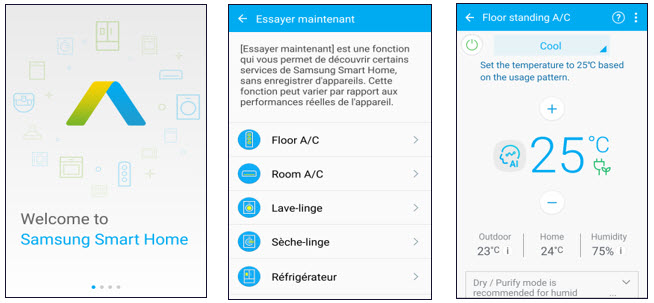
\includegraphics[scale=0.9]{samsung.jpg}
\caption{L'application Samsung Smart Home}
\label{fig:fig1}
\end{figure}
Avec plus de 1 million de téléchargements recensés à ce jour, l’application « Samsung Smart Home » est une référence en terme d’application de domotique et IOT.
Cette application permet aux utilisateurs de se connecter facilement avec divers appareils ménagers, y compris le réfrigérateur, machine à laver, climatiseur, four, aspirateur à vide et plus à travers vos smartphones permettant de surveiller et contrôler les appareils électroménagers Samsung sur la route et profiter des services utiles, y compris vérification de l'état, le contrôle de l'appareil, vue sur la maison, et le soutien à la clientèle.\\
Par contre, on remarque l’absence de quelque service comme :
\begin{itemize}
\item La possibilité de contrôler l’arrosage du jardin grâce à un système d’arrosage automatique communiquant directement avec son smartphone ou son PC.
\item La possibilité de contrôler les lampes et les volets pour plus de confort et une bonne gestion de l’énergie de la maison.
\item La possibilité de mieux renforcer son système de sécurité dans le cas d’un intrus ou d’un incendie et même une fuite de gaz avec un système d’alarme plus propice et plus évolué.
\end{itemize}


\section{Analyse Préalable}
On a commencé par une étude de faisabilité du projet d'une manière globale et simple qui centre sur les besoins des utilisateurs du système. En effet, avant de commencer l’étude préalable, il faut bien comprendre le système et ses intérêts.
On a commencé par une étude de faisabilité du projet d'une manière globale et simple qui centre sur les besoins des utilisateurs du système. En effet, avant de commencer l’étude préalable, il faut bien comprendre le système et ses intérêts. \\
\textbf{C’est quoi exactement ? } \\
La domotique c'est l'informatique appliquée à l'ensemble des systèmes de régulation, de gestion, de communication et de sécurité concernant l'habitat et les tâches de la vie quotidienne. \\
\textbf{Quel est son but ?} \\
La domotique permet d'améliorer le Confort, la Sécurité et la Fonctionnalité de l'habitat. \\
\textbf{Quand intervient-elle ?} \\
Lors de l'utilisation d'appareils électriques. \\
\textbf{Qui peut en avoir besoin ?} \\
La domotique s'adresse au simple bricoleur ainsi qu'à toute personne ayant besoin d'automatisation dans la maison (pour les handicapés par exemple) \\
\textbf{Où pouvons-nous l’utiliser ? } \\
On peut l'utiliser dans l'habitat.\\
\textbf{Comment ça fonctionne ? } \\
La domotique est basée sur la mise en réseau des différents appareils électriques de la maison. Les informations passent par le réseau électrique. \\

\bigskip

\section{Analyse des Besoins}

\subsection{Besoins Non Fonctionnels}
\begin{itemize}
    \item \textbf{Matériel} : Le système doit être compatible à la maison dans laquelle le système va être implémenté. Ainsi, l’application reliée à ce système doit être supporté par les appareils de l’utilisateur.
    \item \textbf{La Confidentialité} : L’authentification se fait par l’administrateur qui peut changer les paramètres par défaut en entrant son pseudo et son mot de passe. D’autre part on trouve un autre mode qui ne nécessite pas l’authentification qui est utilisé, par exemple, par les enfants dont le but de ne pas toucher les paramètres par défaut.
    \item \textbf{La Simplicité} : Le système doit être simple à utiliser, offrant des interfaces qui facilitent l’accès et la modification des paramètres et impressionnantes à voir.
Comportements en cas de panne : Le système est doté d'un utilitaire de détection de panne ainsi qu'une éventuelle correction. Pour les pannes persistantes, les appareils visent à informer l'utilisateur des erreurs produites en lui cédant des alertes.

    \item \textbf{Sécurité} : Le système doit crypter tous les données enregistrés, et doit avoir un par-feu pour interdir les périphériques inconnus à se connecter.
    
    \item \textbf{Prix} : Il comprend le coût de l’installation électrique, des logiciels de supervision et de l’intervention d’un expert pour la configuration et l’adaptation du système.
    \item \textbf{Facilité de déploiment} : La configuration doit être accessible à des personnes non-expertes en domotique pour adapter le système à l’utilisateur dépendant dont les besoins peuvent évoluer rapidement.
    
    \item \textbf{Évolutivité} : Des nouveaux protocoles de “haut niveau” doivent pouvoir être intégrés sans avoir à modifier le travail de conception initial selon la demande du client.
Notre futur objectif : est de veiller sur les personnes ayant des handicaps moteurs, visuels auditifs ou cognitifs ainsi que sur les personnes âgées, dans le cadre du maintien à domicile.
\end{itemize}

\subsection{Besoins Fonctionnels}
Le système domotique offre des diverses fonctionnalités à l’utilisateur pour lui assurer la sécurité, la flexibilité et le confort. \\

\begin{itemize}

\item \textbf{Contrôle du bâtiment, supervision :} 
Visualiser et exploiter votre bâtiment en temps réel, afin de piloter toutes les installations techniques, de faire face aux besoins énergétiques, d’établir une maintenance préventive.

\item \textbf{Gestion des consommations énergétiques :}
Mesurer et enregistrer tous les consommations électriques, thermique, hydraulique, garder la maîtrise des ressources et des contrats.

\item \textbf{Gestion des apports naturels, Façade bioclimatique et dynamique :}
Automatiser les stores en fonction des conditions climatiques, afin optimiser la lumière du jour et contrôler les échanges thermiques. 

\item \textbf{Contrôle des éclairages, Mise en valeur du bâtiment :}
Une régulation active permet d’économiser de 20 \% à 60 \% de l’électricité utilisée pour l’éclairage, en fonction de la saison, de la météo et de l’implantation du bâtiment.

\item \textbf{Régulation et Optimisation de la température :}
En fonction de l’occupation, de l’activité et des conditions climatiques, un contrôle total des équipements de Chauffage, de ventilation et de climatisation.

\item \textbf{Mesures thermiques et climatiques :}
Prise en charges des données météo, de la structure et de l’inertie du bâtiment pour anticiper les besoins et optimiser le confort thermique. 


\item \textbf{Contrôle et visualisation des installations :}
Surveiller la disponibilité de vos installations, être informé en local ou à distance, ajuster au juste besoin vos consignes, vos programmes horaires.
\end{itemize}




\section*{Conclusion}
L'objectif de cette partie était de présenter les fondements théoriques du projet en se basant en premièr lieux sur l'étude des applications similaires existants sur le marché, et dans un deuxième lieux sur un analyse des besoins fonctionnels et non fonctionnels de notre application.


%==============================================================================
\end{spacing}

\part{Partie 2}

\setcounter{chapter}{1}
\chapter{Conception}
\minitoc %insert la minitoc
\graphicspath{{Chapitre2/figures/}}

%\DoPToC

%==============================================================================
\pagestyle{fancy}
\fancyhf{}
\fancyhead[R]{\bfseries\rightmark}
\fancyfoot[R]{\thepage}
\renewcommand{\headrulewidth}{0.5pt}
\renewcommand{\footrulewidth}{0pt}
\renewcommand{\chaptermark}[1]{\markboth{\MakeUppercase{\chaptername~\thechapter. #1 }}{}}
\renewcommand{\sectionmark}[1]{\markright{\thechapter.\thesection~ #1}}

\begin{spacing}{1.2}
%==============================================================================

\section*{Introduction}
Vu que nous avons achevé la première phase (Analyse) du cycle de développement, nous aborderons dans ce chapitre la deuxième phase (Conception) qui se concentre essentiellement sur la définition de l’architecture du système ainsi que sur l’analyse et la conception des besoins et des exigences des utilisateurs.  L’activité d’analyse et de conception permet de traduire les besoins fonctionnels et les contraintes issues du cahier des charges et de la spécification des exigences dans un langage plus professionnel et compréhensible par tous les individus intervenants dans la réalisation et l’utilisation de l’application

\newpage
\section{Diagrammes}
\subsection{Diagramme de cas d'utilisation}
Le diagramme de cas d'utilisation ( \autoref{fig:fig2} ) est utilisé pour donner une vision globale du comportement fonctionnel du système .

\begin{figure}[H]\centering
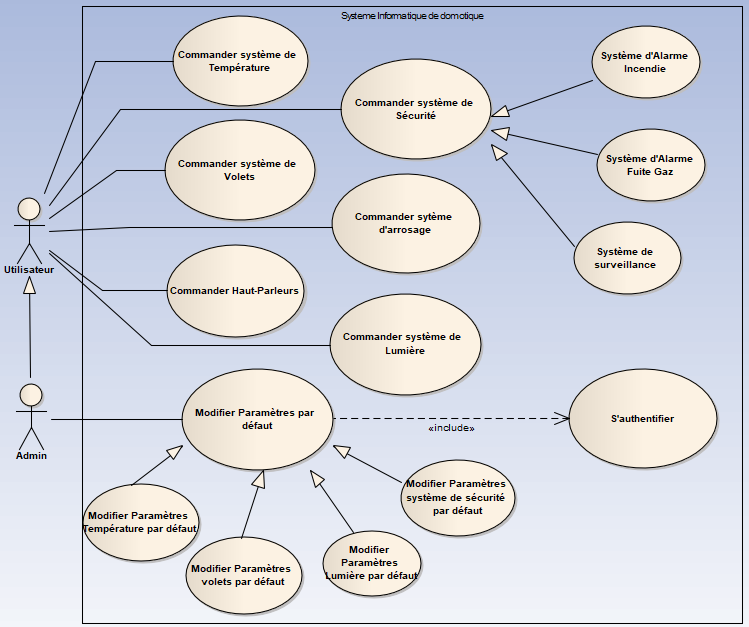
\includegraphics[scale=0.9]{1.png}
\caption{Diagramme de cas d'utilisations}
\label{fig:fig2}
\end{figure}




\begin{table}[H]
	\centering
	\caption{Classement des cas d’utilisation}
	\footnotesize
	\begin{tabularx}{\linewidth}{|>{\bfseries \vspace*{\fill}}X ||>{\centering{}\vspace*{\fill}}X|>{\vspace*{\fill}}X<{\centering{}}|}	
			\hline 
			Cas d’utilisation & \bfseries Priorité & \bfseries Risque\\
			\hline \hline
			Commander Système de Température		&	Moyenne	&	Moyen	\\
			Commander Système de Lumière		&	Moyenne	&	Moyen	\\
			Commander Système des Volets		&	Moyenne	&	Moyen	\\
			Commander Système de Sécurité		&	Moyenne	&	Moyen	\\
			Commander Système d’arrotissage		&	Moyenne	&	Moyen	\\
			Commander Haut-Parleurs		&	Faible	&	Moyen	\\
			Paramétrer Système de Sécurité		&	Haute	&	Haut	\\
			Paramétrer les Volets		&	Haute	&	Bas	\\
			Paramétrer la Lumière		&	Haute	&	Bas	\\
			Paramétrer la Température		&	Haute	&	Bas	\\
			S’authentifier		&	Faible	&	Haut	\\
			\hline
	\end{tabularx}
	\label{tab:exple}
\end{table}


\subsection{Diagrammes de Classes}
\subsubsection{Système de Température}

\begin{figure}[H]\centering
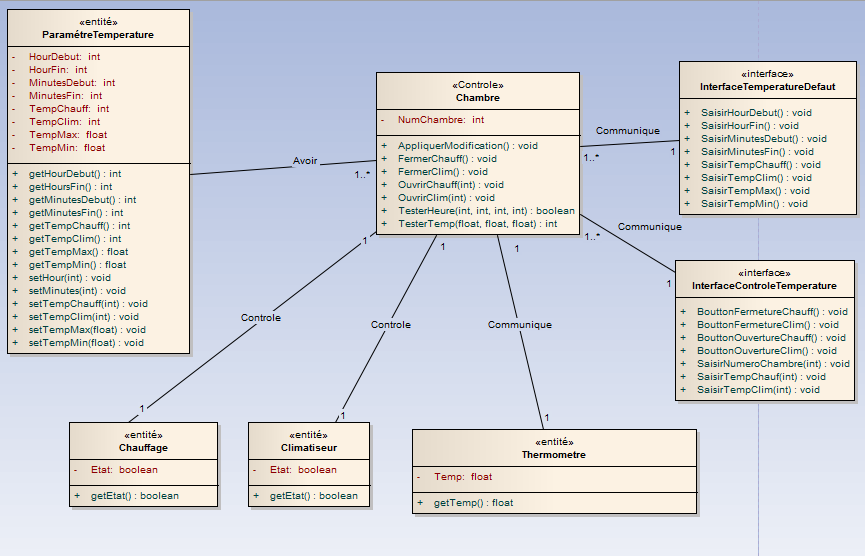
\includegraphics[scale=0.8]{2.png}
\caption{Diagramme de Classes du Système de Température}
\label{fig:fig3}
\end{figure}

\subsubsection{Système de Sécurité}

\textbf{Système de caméra de surveillance}

\begin{figure}[H]\centering
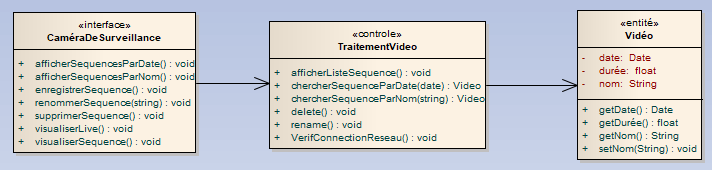
\includegraphics[scale=0.9]{3.png}
\caption{Diagramme de Classes du Système de caméra de surveillance}
\label{fig:fig3}
\end{figure}

\textbf{Système d’alarme d’incendie}

\begin{figure}[H]\centering
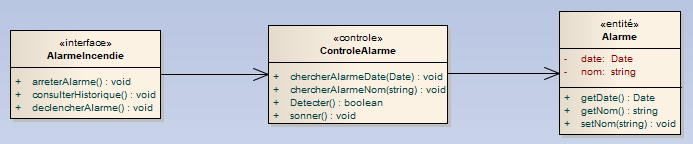
\includegraphics[scale=0.9]{4.png}
\caption{Diagramme de Classes du Système d’alarme d’incendie}
\label{fig:fig3}
\end{figure}

\textbf{Système d’alarme de fuite de Gaz}

\begin{figure}[H]\centering
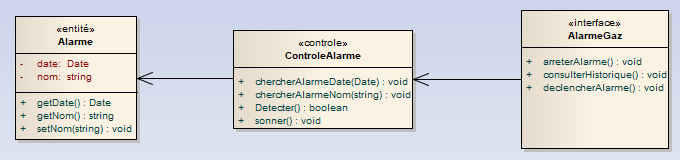
\includegraphics[scale=0.9]{5.png}
\caption{Diagramme de Classes du Système d’alarme de fuite de Gaz}
\label{fig:fig3}
\end{figure}

\subsubsection{Système de Volets}
\begin{figure}[H]\centering
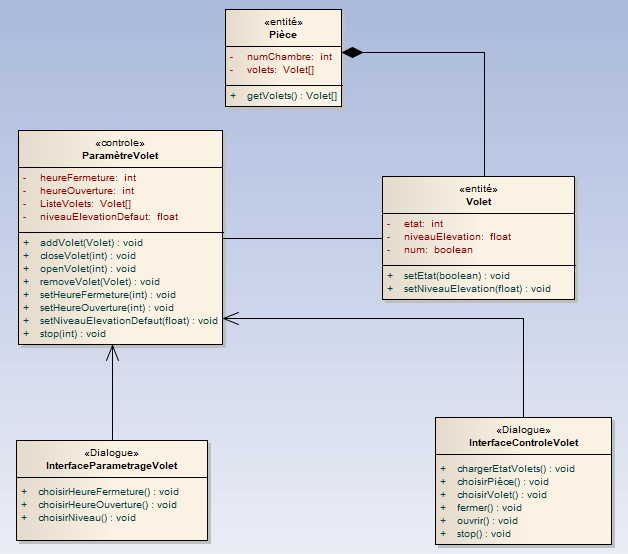
\includegraphics[scale=0.9]{6.png}
\caption{Diagramme de Classes du Système de Volets}
\label{fig:fig3}
\end{figure}

\subsubsection{Système de Lumière}
Remarques concernant quelques méthodes du diagramme de classe :
\begin{itemize}
    \item \textbf{debutCompteur :int} c’est la valeur du compteur à partir de laquelle on calcule la consommation d’électricité. 
    \item \textbf{gererConflit() :void} permet la gestion des problèmes si deux éclairages sont contradictoires et propose des suggestions de solutions. 
    \item \textbf{calculerConsommation() :void} permet de calculer la consommation , en effet  elle applique la formule suivante : consommation = numeroCompteur – debutCompteur. \\
    \item \textbf{indiquerFacturePayé () : void} permet d’informer le système que l’utilisateur a payé la facture d’électricité ce qui permet de calculer la consommation en électricité à partir du dernier péage.
    \item \textbf{CalculerDebutCompteur() :void} permet de changer l’attribut debutCompteur par le numero du compteur après un péage.
\end{itemize}

\begin{figure}[H]\centering
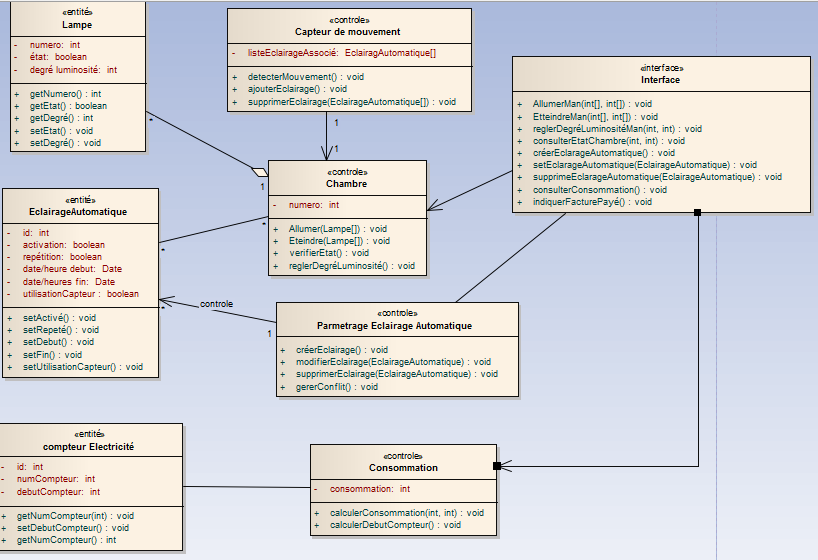
\includegraphics[scale=0.8]{7.png}
\caption{Diagramme de Classes du Système de Lumière}
\label{fig:fig3}
\end{figure}
 
\subsubsection{Système d’arrosage}
\begin{figure}[H]\centering
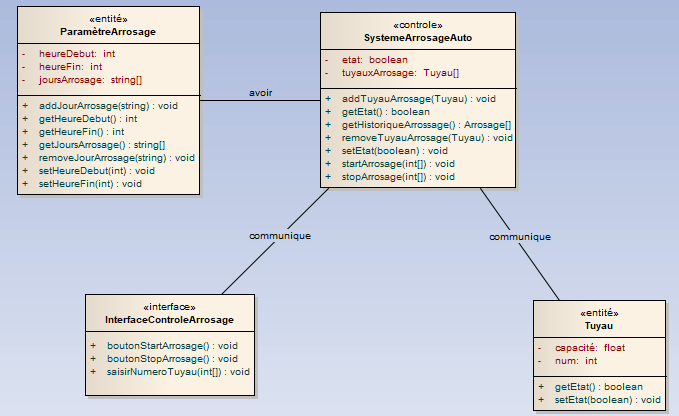
\includegraphics[scale=0.8]{8.png}
\caption{Diagramme de Classes du Système d’arrosage}
\label{fig:fig3}
\end{figure}

\subsubsection{Haut-Parleurs}
\begin{figure}[H]\centering
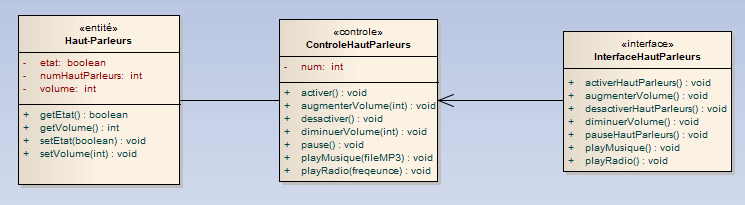
\includegraphics[scale=0.8]{9.png}
\caption{Diagramme de Classes des Haut-Parleurs}
\label{fig:fig3}
\end{figure}

\subsection{Diagramme de Paquetages}

\begin{figure}[H]\centering
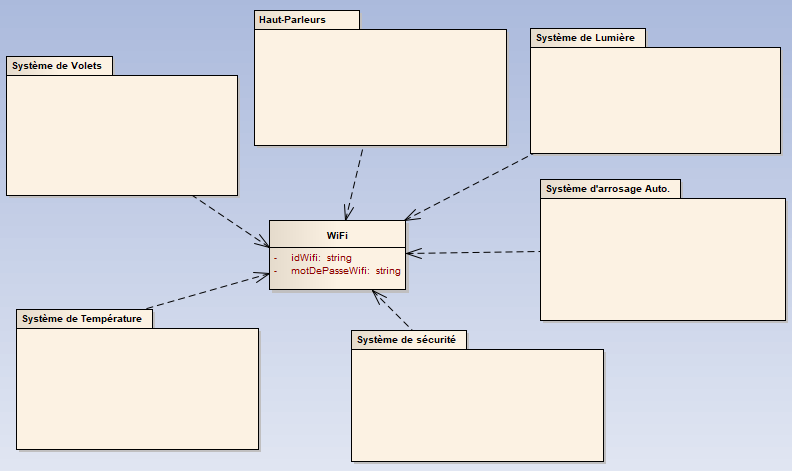
\includegraphics[scale=0.8]{32.png}
\caption{Diagramme de Paquetages}
\label{fig:fig3}
\end{figure}

\newpage

\subsection{Diagrammes de séquence}

\subsubsection{Système de température }

\textbf{Scénario de gestion automatique de la température : }
\begin{figure}[H]\centering
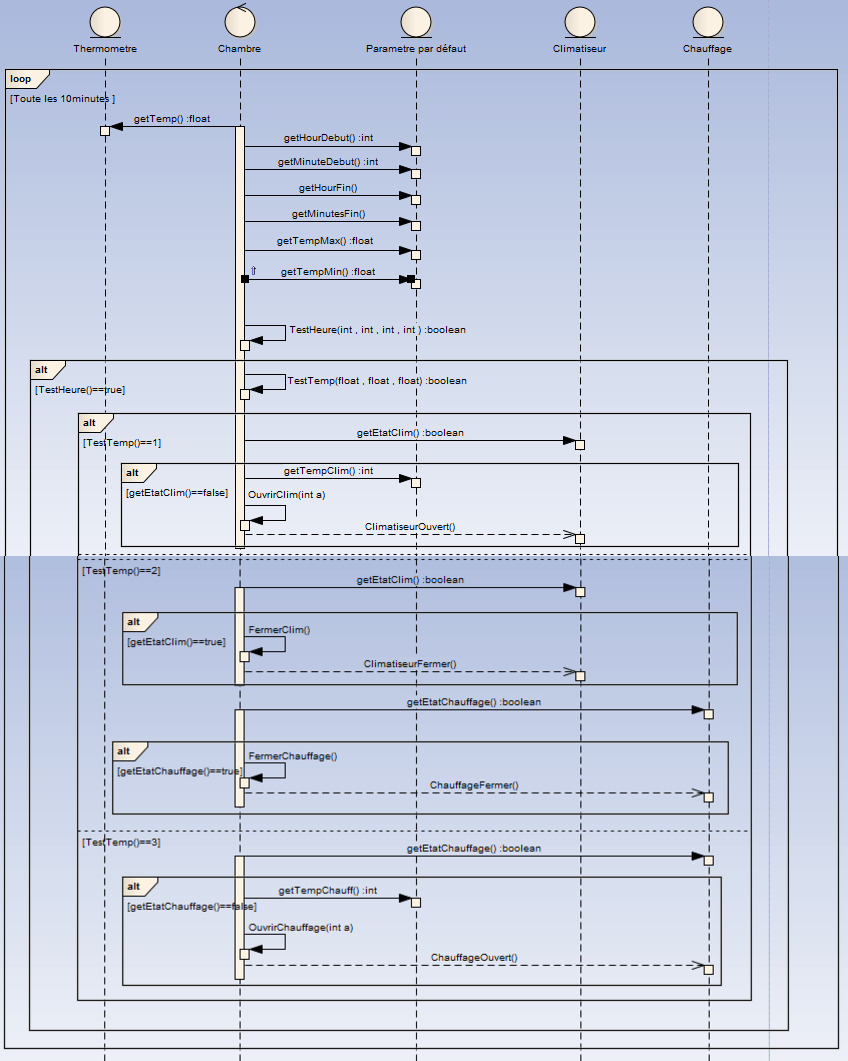
\includegraphics[scale=0.6]{12.jpg}
\caption{Diagramme de Séquence: Gestion automatique de la température}
\label{fig:fig3}
\end{figure}

\bigskip

\textbf{Scénario ouverture climatiseur manuelle : }
\begin{figure}[H]\centering
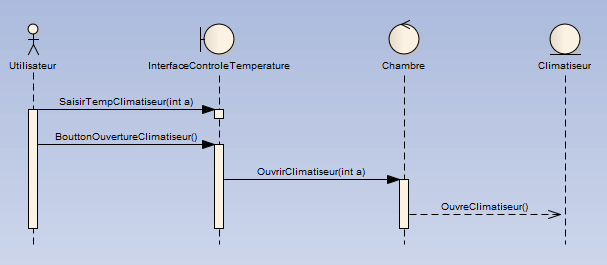
\includegraphics[scale=0.8]{13.png}
\caption{Diagramme de Séquence: Ouverture climatiseur manuelle}
\label{fig:fig3}
\end{figure}

\textbf{Scénario ouverture chauffage manuelle :}
\begin{figure}[H]\centering
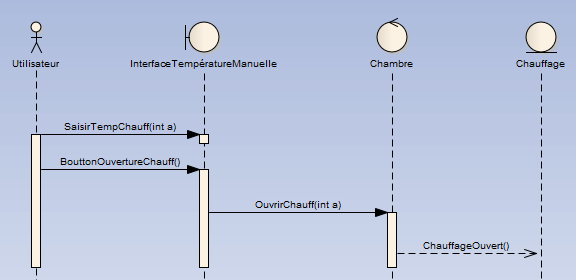
\includegraphics[scale=0.8]{14.png}
\caption{Diagramme de Séquence: Ouverture chauffage manuelle}
\label{fig:fig3}
\end{figure}

\newpage

\subsubsection{Système de lumière}

\textbf{Scénario d’éclairage manuel :}
\begin{figure}[H]\centering
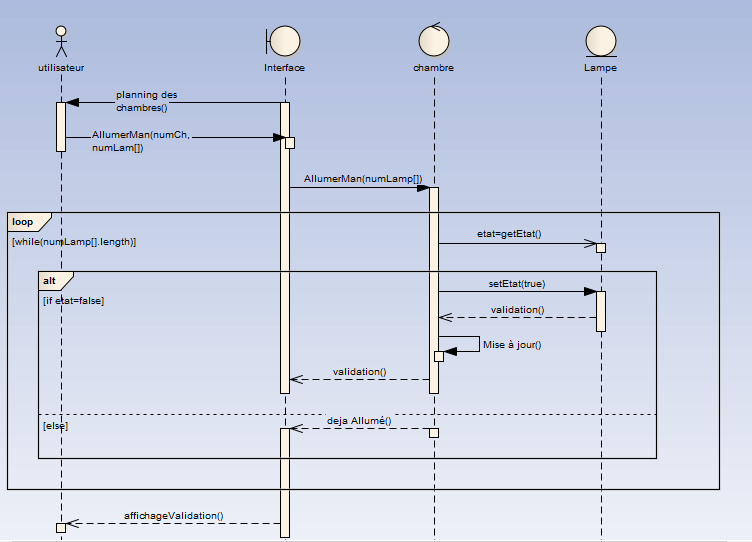
\includegraphics[scale=0.9]{15.png}
\caption{Diagramme de Séquence: Eclairage manuel}
\label{fig:fig3}
\end{figure}

\newpage

\textbf{Scénario d’extinction manuel de lumière :}
\begin{figure}[H]\centering
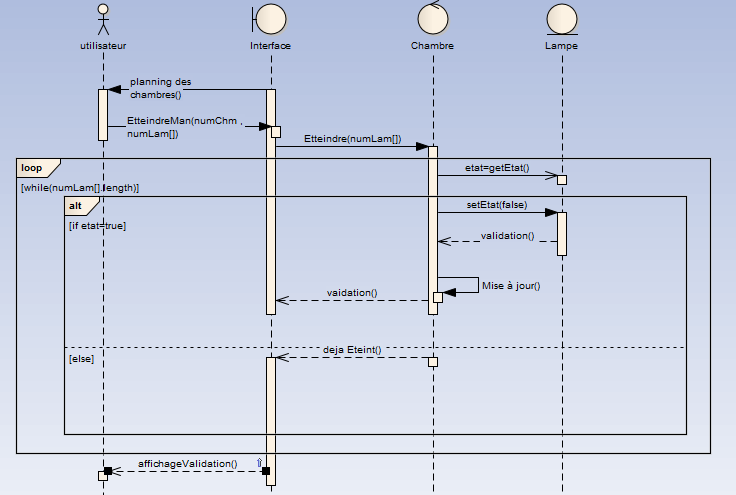
\includegraphics[scale=0.7]{16.png}
\caption{Diagramme de Séquence: Extinction manuel de lumière}
\label{fig:fig3}
\end{figure}

\newpage

\textbf{Scénario de consultation de la consommation de lumière :}
\begin{figure}[H]\centering
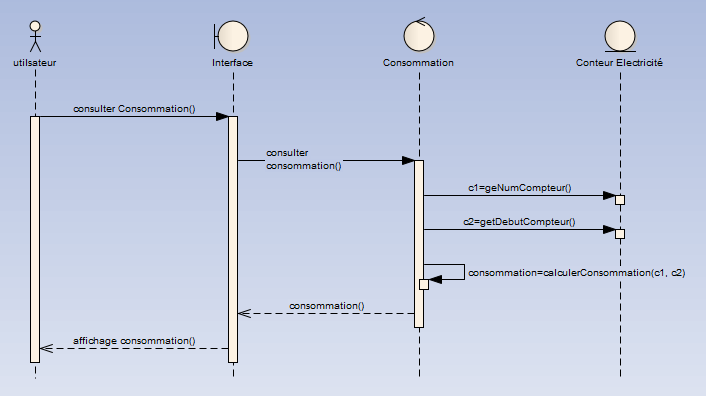
\includegraphics[scale=0.8]{17.png}
\caption{Diagramme de Séquence: Consultation de la consommation de lumière}
\label{fig:fig3}
\end{figure}
 
 
 \textbf{Scénario de réglage de degré de luminosité :}
\begin{figure}[H]\centering
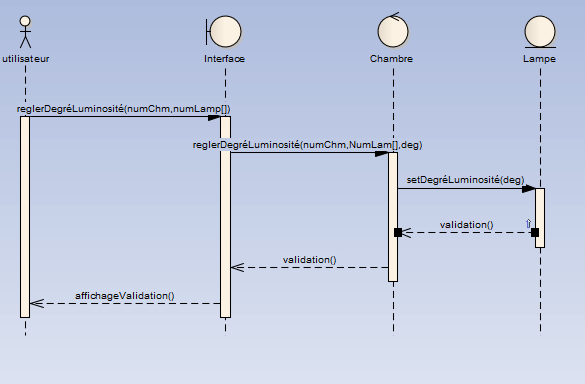
\includegraphics[scale=0.8]{18.png}
\caption{Diagramme de Séquence: Réglage de degré de luminosité}
\label{fig:fig3}
\end{figure}

\newpage
 
 \textbf{Scénario de création d’éclairage automatique :}
\begin{figure}[H]\centering
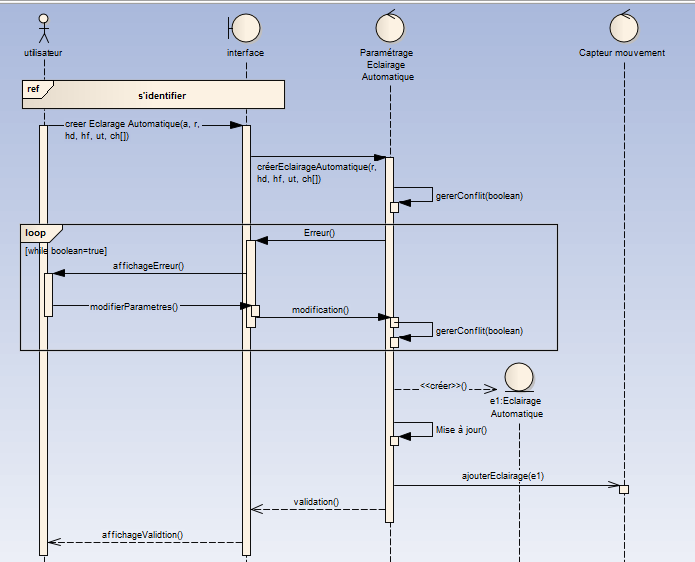
\includegraphics[scale=0.9]{19.png}
\caption{Diagramme de Séquence: Création d’éclairage automatique}
\label{fig:fig3}
\end{figure}

\newpage
 
 \textbf{Scénario de suppression d’un éclairage automatique :}
\begin{figure}[H]\centering
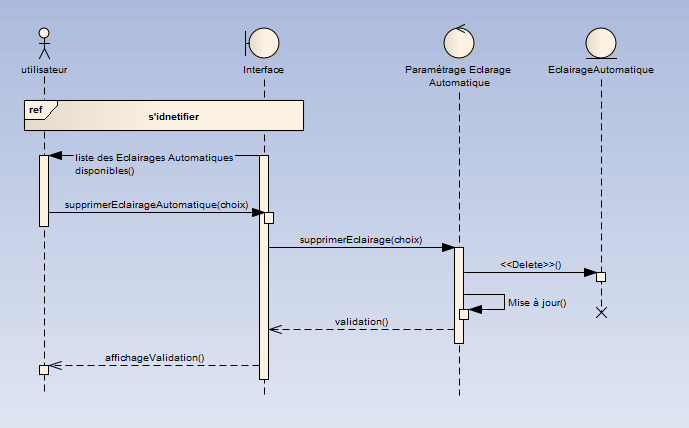
\includegraphics[scale=1]{20.png}
\caption{Diagramme de Séquence: Suppression d’un éclairage automatique}
\label{fig:fig3}
\end{figure}
 
 \newpage
 
 \textbf{Scénario de modification d’un éclairage automatique :}
\begin{figure}[H]\centering
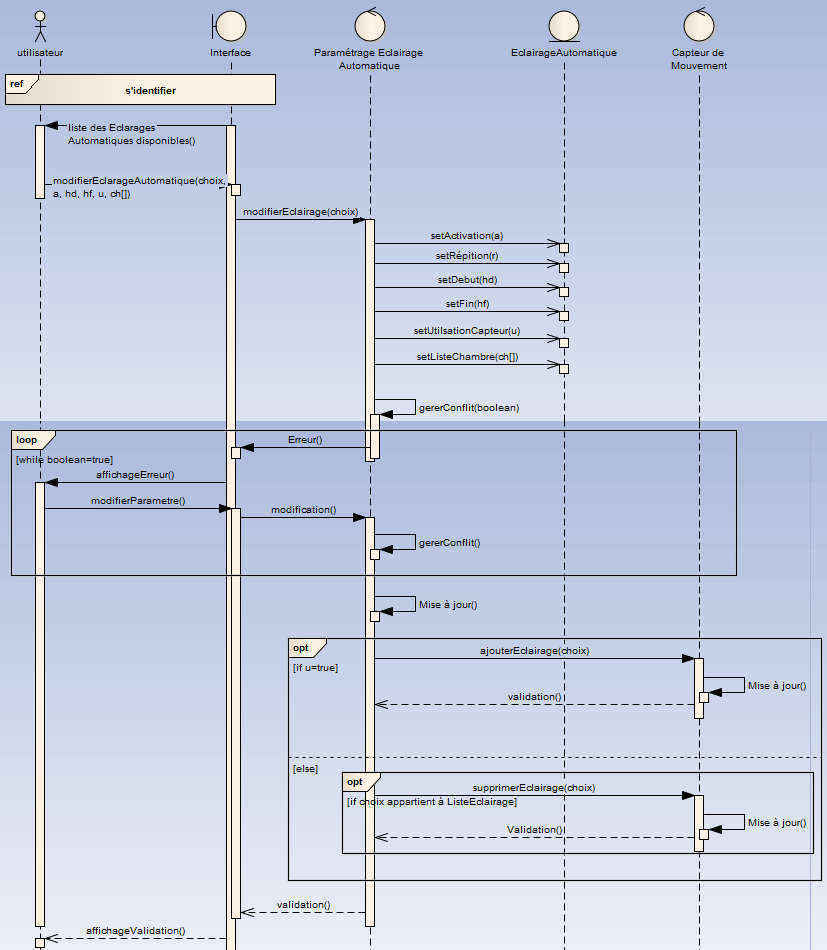
\includegraphics[scale=0.8]{23.png}
\caption{Diagramme de Séquence: Modification d’un éclairage automatique}
\label{fig:fig3}
\end{figure}
 
\subsubsection{Système des volets }

\textbf{Scénario de Fermeture des Volets :} \\
L’utilisateur peut aussi fermer manuellement les volets. lorsque l’utilisateur choisie « fermeture volet » , la liste des chambres s’affiche  ,il choisie celle qui est concerné  ainsi que  les volets qu’il veut les fermer ..si la fermeture a etteint le niveau max sans avoir toucher le bouton « stop » alors la base de donnée se mit à jours et l’etat du volet devient « fermé » sinon il reste à l’etat « ouvert » . 

\begin{figure}[H]\centering
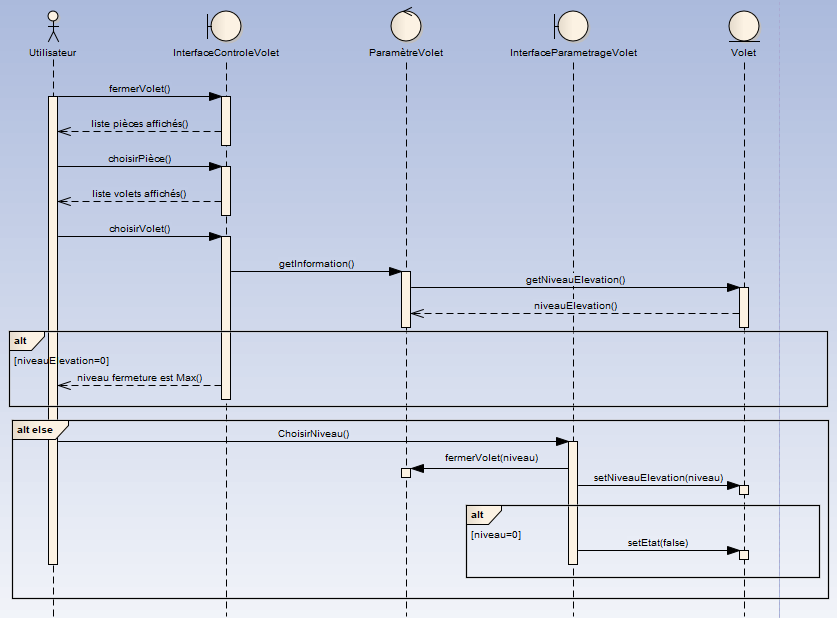
\includegraphics[scale=0.8]{24.png}
\caption{Diagramme de Séquence: Fermeture des Volets}
\label{fig:fig3}
\end{figure}

\newpage

\textbf{Scénario de Ouverture des Volets :} \\
Pour des raisons du confort , notre système assure un control à distance pour tous les volets , il suffit just d’ouvrir l’application et choisir « volet » puis « ouvrir volets » , une liste des chambres s’affiche  , l’utilisateur selectionne la chambre desiré,la liste des volets de ette chambre s’affiche,il selectionne ainsi tous les volets qu’il veut les ouvrir . apres ressemblage d’information depuis la base de donnée , un affichage du dernier etat des volets et leurs niveaux d’elevation apparait. en touchant  le bouton « ouvrir » les volets s’ouvrent jusqu’à toucher le bouton « stop » . 
\begin{figure}[H]\centering
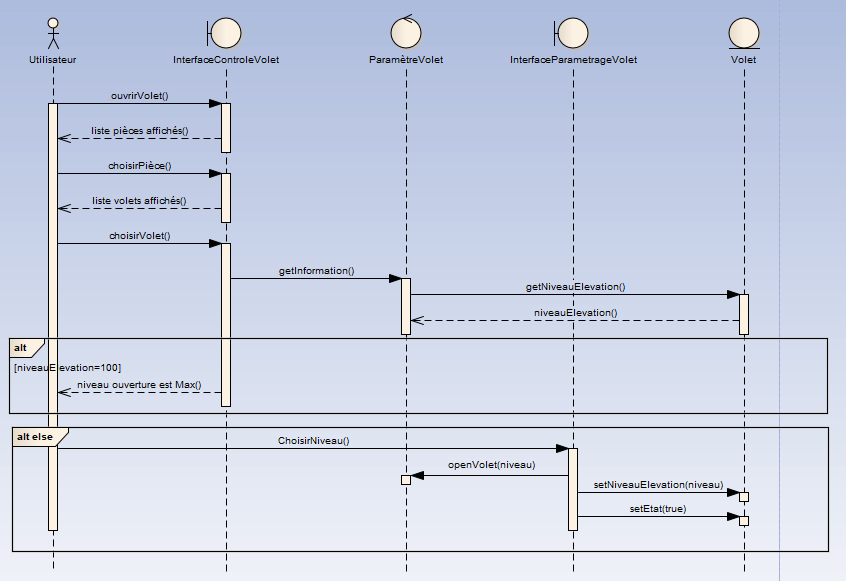
\includegraphics[scale=0.8]{25.png}
\caption{Diagramme de Séquence: Ouverture des Volets}
\label{fig:fig3}
\end{figure}

\newpage

\subsection{Diagrammes d’état-Transition}

\subsubsection{Activer/desactiver mode automatique des volets et d’arrosage Auto.}
Le système offre le choix entre l’activation ou la désactivation du mode automatique.
Il suffit juste de toucher le bouton « on/off » pour changer le mode a chaque fois.
\begin{figure}[H]\centering
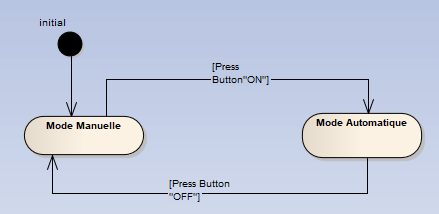
\includegraphics[scale=0.8]{26.png}
\caption{Diagramme d'état-Transition : Gestion des volets}
\label{fig:fig3}
\end{figure}

\subsubsection{Gestion des Haut-Parleurs}
\begin{figure}[H]\centering
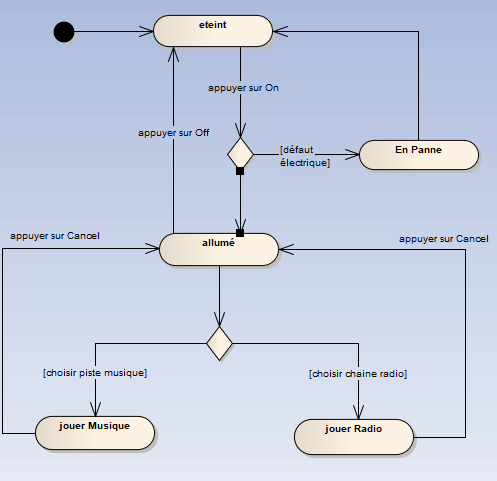
\includegraphics[scale=0.8]{27.png}
\caption{Diagramme d'état-Transition : Gestion des Haut-Parleurs}
\label{fig:fig3}
\end{figure}
 
 
 
\subsection{Diagramme d’activité }
\subsubsection{Système de caméra de surveillance }
Le vidéo de surveillance doit permettre une détection automatique de mouvement afin éventuellement de déclencher une alarme qui sera par la suite transmise vers le réseau GSM pour envoyer un SMS, ou transmise vers le réseau Wifi pour envoyer un mail pour informer l’utilisateur de ce que se passe en recevant une séquence vidéo.  

\begin{figure}[H]\centering
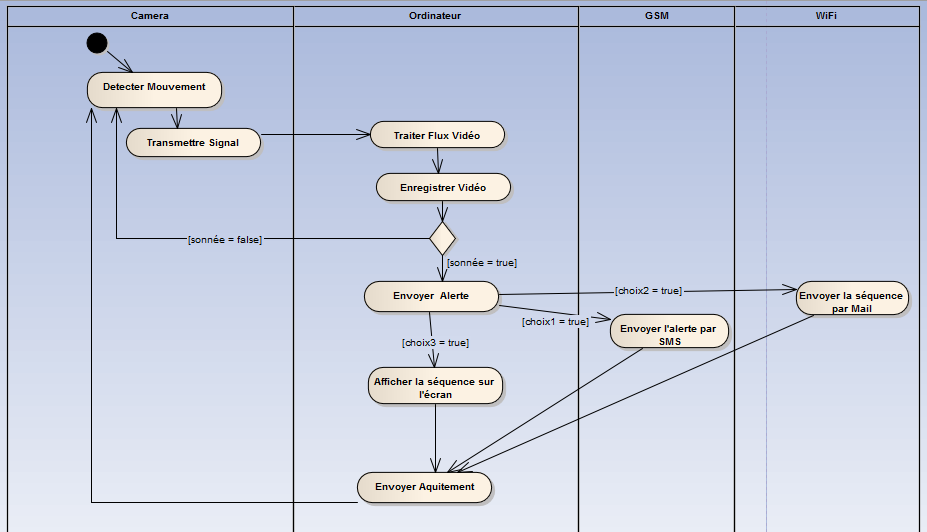
\includegraphics[scale=0.7]{28.png}
\caption{Diagramme d'Activité : Gestion des Caméras de surveillance}
\label{fig:fig3}
\end{figure}
 
 \newpage
\subsubsection{Système d’alarme d’incendie}
Cet appareil doit permettre une détection automatique d’incendie pour provoquer des actions immédiates.
En effet, un système d’alarme qui va se déclencher, avec une pulvérisation de l’eau qui reste 2 minutes puis le système envoie un SMS au pompier d’une part et aux propriétaires d’autre part. 

\begin{figure}[H]\centering
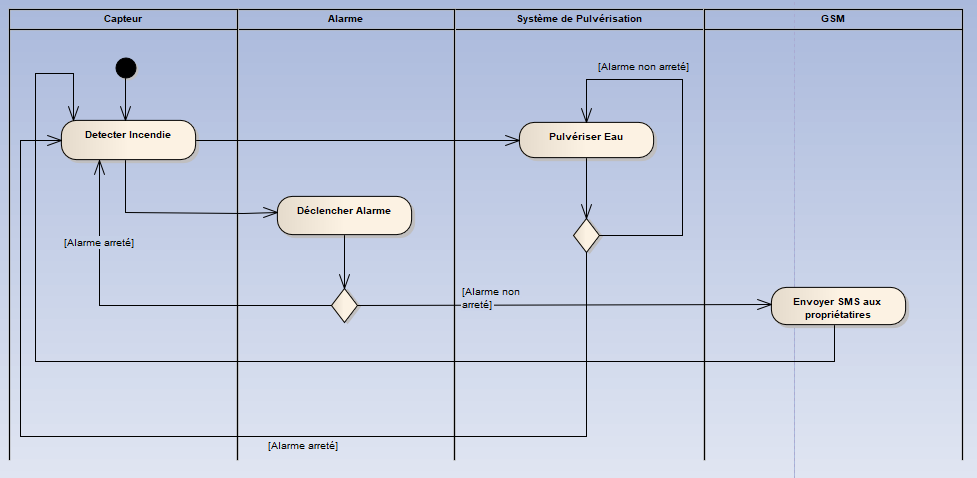
\includegraphics[scale=0.7]{29.png}
\caption{Diagramme d'Activité : Gestion d'Alarme d'incendie}
\label{fig:fig3}
\end{figure} 

\newpage
 
\subsubsection{Système d’alarme Fuite Gaz}
Cet appareil doit permettre une détection automatique d’une fuite de gaz pour provoquer des actions immédiates.
En effet, un système d’alarme qui va se déclencher puis le système envoie une notification aux propriétaires.
\begin{figure}[H]\centering
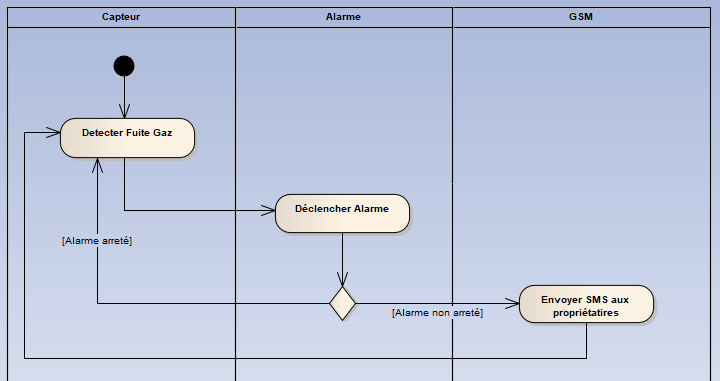
\includegraphics[scale=0.9]{30.png}
\caption{Diagramme d'Activité : Gestion d'Alarme Fuite Gaz}
\label{fig:fig3}
\end{figure} 

\subsubsection{Système d’arrosage Automatique}
\begin{figure}[H]\centering
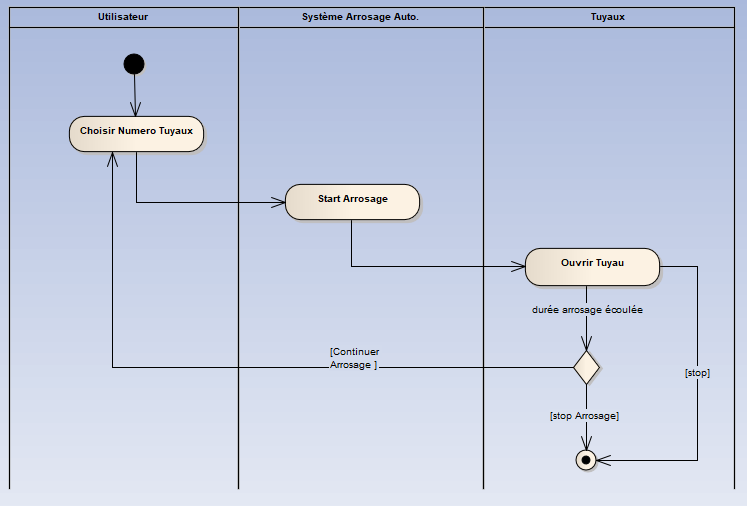
\includegraphics[scale=0.8]{31.png}
\caption{Diagramme d'Activité : Gestion d'Arrosage Automatique}
\label{fig:fig3}
\end{figure} 

\newpage

\subsection{Diagramme de Navigation}
 Permet de naviguer entre les éléments d’un système (les interfaces de l’application dans notre cas) :
 
 \begin{figure}[H]\centering
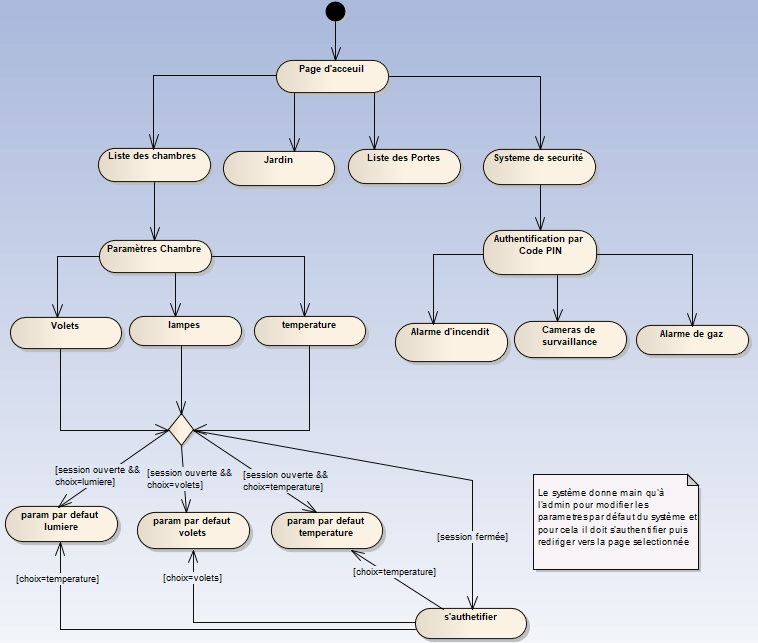
\includegraphics[scale=0.8]{33.png}
\caption{Diagramme Navigation}
\label{fig:fig3}
\end{figure} 

 
\section*{Conclusion}
Dans ce chapitre, nous avons utilisé le langage de modélisation UML (Unified Modeling Language) pour établir les différents diagrammes, ce qui nous a permis d’extraire d’une part les différentes fonctionnalités que doit offrir notre application aux différents acteurs, et d’autre part de concevoir les classes .





%==============================================================================
\end{spacing}


\setcounter{chapter}{2}
\chapter{R�alisation}
\minitoc %insert la minitoc
\graphicspath{{Chapitre3/figures/}}

%\DoPToC
%==============================================================================
\pagestyle{fancy}
\fancyhf{}
\fancyhead[R]{\bfseries\rightmark}
\fancyfoot[R]{\thepage}
\renewcommand{\headrulewidth}{0.5pt}
\renewcommand{\footrulewidth}{0pt}
\renewcommand{\chaptermark}[1]{\markboth{\MakeUppercase{\chaptername~\thechapter. #1 }}{}}
\renewcommand{\sectionmark}[1]{\markright{\thechapter.\thesection~ #1}}

\begin{spacing}{1.2}

%==============================================================================
\section*{Introduction}
Ce chapitre porte sur la partie pratique ainsi que la bibliographie.

\section{Outils et langages utilis�s}
L'�tude technique peut se trouver dans cette partie, comme elle peut �tre faite en
parall�le avec l'�tude th�orique (comme le sugg�re le mod�le 2TUP).
Dans cette partie, il faut essayer de convaincre le lecteur de vos choix en termes de
technologie. Un �tat de l'art est souhait� ici, avec un comparatif, une synth�se et un choix 
d'outils, m�me tr�s brefs.
\section{Pr�sentation de l'application}
Il est tout � fait normal que tout le monde attende cette partie pour coller � souhait toutes les images
correspondant aux interfaces diverses de l'application si ch�re � votre coeur, mais
abstenez vous! Il FAUT mettre des imprime �crans, mais bien choisis, et surtout, il faut les sc�nariser : Choisissez un sc�nario d'ex�cution, par exemple la cr�ation d'un 
nouveau client, et montrer les diff�rentes interfaces n�cessaires pour le faire, en
expliquant bri�vement le comportement de l'application. Pas trop d'images, ni trop de
commentaires : concis, encore et toujours.

�vitez ici de coller du code : personne n'a envie de voir le contenu de vos classes.
Mais  vous  pouvez ins�rer des snippets (bouts de code) pour montrer certaines
fonctionnalit�s \cite{YOUSFI2015}\cite{Latex}, si vous en avez vraiment besoin. Si vous voulez montrer une partie de votre code, les �tapes d'installation ou de configuration, vous pourrez les mettre dans l'annexe.
\subsection{Exemple de tableau}

Vous pouvez utiliser une description tabulaire d'une �ventuelle comparaison entre les travaux existants. Ceci est un exemple de tableau: Tab \ref{tab:exple}.

\begin{table}[ht]
	\centering
	\caption{Tableau comparatif}
	\footnotesize
	\begin{tabularx}{\linewidth}{|>{\bfseries \vspace*{\fill}}X ||>{\centering{}\vspace*{\fill}}X|>{\centering{}\vspace*{\fill}}X|>{\centering{}\vspace*{\fill}}X|>{\vspace*{\fill}}X<{\centering{}}|}	
			\hline 
			& \bfseries Col1 & \bfseries Col2 &\bfseries Col3 &\bfseries Col4\\
			\hline \hline
			Row1		&		&	X	&		&		\\
			Row2		&	X	&		&		&		\\
			Row3		&	X	&	X	&	X	&	X	\\
			Row4		&	X	&		&	X	&	X	\\
			Row5		&	X	&		&	X	&	X	\\
			Row6		&	X	&		&	X	&	X	\\
			Row7		&	X	&		&	X	&		\\
			Row8		&	X	&	X	&	X	&		\\
			\hline
	\end{tabularx}
	\label{tab:exple}
\end{table}

\subsection{Exemple de Code}
Voici un exemple de code Java, avec coloration syntaxique \ref{code:java}.

\begin{lstlisting}[rulecolor=\color{white}]
\end{lstlisting}

\begin{lstlisting}[label=code:java,caption=Helloworld Java,language=java]
	public class HelloWorld {
	//la m�thode main
    public static void main(String[] args) {
        System.out.println("Hello, World");
    }

}
\end{lstlisting}

\section{Remarques sur la bibliographie}
Votre bibliographie doit r�pondre � certains crit�res, sinon, on vous fera encore et
toujours la remarque dessus (et parfois, m�me si vous pensez avoir tout fait comme il
 faut, on peut vous faire la remarque quand m�me : chacun a une conception tr�s
personnelle de comment une bibliographie devrait �tre).\\
\begin{itemize}
\item Une bibliographie dans un bon rapport doit contenir plus de livres et d'articles 
que de sites web : apr�s tout c'est une biblio. Privil�giez donc les ouvrages
reconnus et publi�s pour vos d�finitions, au lieu de sauter directement sur le premier article wikipedia;
 \item Les �l�ments d'une bibliographie sont de pr�f�rence class�s par ordre
alphab�tique, ou par th�mes (et ordre alphab�tique pour chaque th�me);
\item Une entr�e bibliographique doit �tre sous la forme suivante :
\begin{itemize}
\item Elle doit contenir un identifiant unique: repr�sent� soit par un num�ro
[1] ou par le nom du premier auteur, suivi de l'ann�e d'�dition [Kuntz, 1987];
\item Si c'est un livre : Les noms des auteurs, suivi du titre du livre, de l'�diteur, 
ISBN/ISSN, et la date d'�dition;
\item Si c'est un article : Les noms des auteurs, le titre , le journal ou la
conf�rence, et la date de publication;
\item Si c'est un site web ou un document �lectronique : Le titre, le lien et la date 
de consultation;
\item Si c'est une th�se : nom et pr�nom, titre de la th�se, universit� de
soutenance, ann�e de soutenance, nombre de pages;
\item Exemples : 
\begin{description}
\item $[Bazin, 1992]$ BAZIN R., REGNIER B. Les traitements antiviraux et leurs essais
th�rapeutiques. Rev. Prat., 1992, 42, 2, p.148-153.\\
\item $[Anderson,1998]$ ANDERSON P.JF. Checklist of criteria used for evaluation of metasites.
[en ligne]. Universit� du Michigan, Etats Unis. Site disponible sur :\\
http://www.lib.umich.edu/megasite/critlist.html.(Page consult�e le 11/09/1998).
\end{description}
\item Dans le texte du rapport, on doit obligatoirement citer la r�f�rence en  faisant appel � son identifiant, juste apr�s avoir utilis� la citation. Si ceci n'est pas fait dans les r�gles, on peut �tre accus� de plagiat.
\end{itemize} 
\end{itemize} 

\section*{Conclusion}
Voil�.

%==============================================================================
\end{spacing}


\backmatter
\pagestyle{fancy}
\fancyhf{}
\renewcommand{\chaptermark}[1]{\markboth{Conclusion Générale et Perspectives}{}}
\fancyhead[R]{Conclusion Générale et Perspectives}
\fancyfoot[R]{\thepage}
\renewcommand{\headrulewidth}{0.5pt}
\renewcommand{\footrulewidth}{0pt}
\chapter{Conclusion Générale et Perspectives}
%==============================================================================
\pagestyle{fancy}
\fancyhf{}
\fancyhead[R]{\bfseries\rightmark}
\fancyfoot[R]{\thepage}
\renewcommand{\headrulewidth}{0.5pt}
\renewcommand{\footrulewidth}{0pt}
\renewcommand{\chaptermark}[1]{\markboth{\MakeUppercase{\chaptername~\thechapter. #1 }}{}}
\renewcommand{\sectionmark}[1]{\markright{\thechapter.\thesection~ #1}}

\begin{spacing}{1.2}
%==============================================================================

L’objectif de notre projet était de concevoir et de réaliser un système informatique de domotique. Le point de départ de la réalisation de ce projet était une récolte des informations nécessaires pour dresser un état de l’existant, présenter un aperçu sur la problématique. Par la suite, nous nous sommes intéressés à l’analyse et la spécification des besoins qui nous a permis de distinguer les différents acteurs interagissant avec l’application visée. L’objectif de la partie suivante était la conception détaillée, dans laquelle nous avons fixé la structure globale de l’application. Le dernier volet de notre projet était la partie réalisation qui a été consacrée à la présentation des outils du travail et les interfaces les plus significatives de notre application. L’apport de ce travail a été d’une importance très considérable, en effet, il nous a permis : de suivre une méthodologie de travail bien étudié, d’approfondir nos connaissances conceptuelles acquises tout au long de ce semestre en mettant en pratique le formalisme UML à travers un panel large et diversifié de diagrammes et bien maitriser ce concept. \\
La réalisation d’un tel projet, nous a permis d’apprendre et de toucher du doigt une partie de divers aspects du métier de développeur et de celui du concepteur.
\\
Ce travail répond aux besoins préalablement fixés mais il pourra évidemment être amélioré et optimisé par l’ajout de nouvelles fonctionnalités comme la gestion d'autres logement et bâtiments sous la même application.
%==============================================================================
\end{spacing}



\onehalfspacing

\appendix


\end{document}
